\chapter{Méthode et résultats}
\label{chap:methode}

\section{Méthode}

La méthode s'appuie sur le modèle
\begin{equation}
  \label{eq:modele}
  \frac{\mathrm{d}x}{\mathrm{d}t} = -\lambda x, \qquad x(0) = x_0,
\end{equation}
dont la solution est $x(t) = x_0 e^{-\lambda t}$.

\section{Résultats}

La figure~\ref{fig:resultats} et le tableau~\ref{tab:resultats} présentent
les résultats obtenus avec le modèle~\eqref{eq:modele}.

\begin{figure}[htbp]
  \centering
  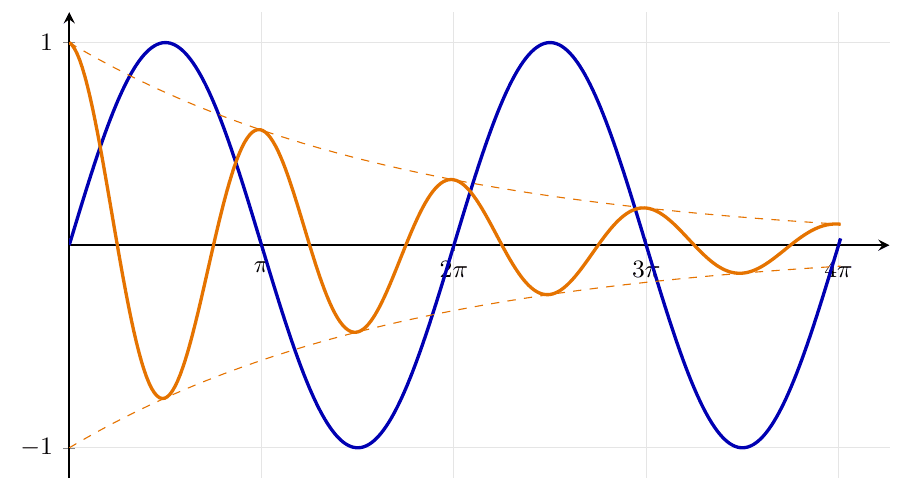
\includegraphics[width=0.75\linewidth]{images/courbes.png}
  \caption{Une image du projet: remplacez-la par vos résultats.}
  \label{fig:resultats}
\end{figure}

\begin{table}[htbp]
  \centering
  \caption{Valeurs estimées du paramètre $\lambda$.}
  \label{tab:resultats}
  \begin{tabular}{lrr}
    \toprule
    Essai & $\lambda$ & Erreur relative (\%) \\
    \midrule
    1 & 0,182 & 1,1 \\
    2 & 0,179 & 0,6 \\
    3 & 0,185 & 2,8 \\
    \bottomrule
  \end{tabular}
\end{table}
